We evaluate the performance of B2B throughout a series of experiments on
controlled synthetic data.
%
The purpose of these experiments is to evaluate the ability of B2B on its
ability to 1) accurately predict independent and identically distributed data,
and 2) recover causal factors when the ground truth is known.

The data generating process for each experiment constructs $n=1000$ training examples
according to the model $Y = (\text{h} XE + N)F$, where $\text{h}$ is a
scalar that modulates the signal-to-noise ratio.
%
Here,
%\begin{itemize} \item $F \in \mathbb{R}^{d_x \times d_y}$ contains entries
%drawn from $\mathcal{N}(0, \sigma^2)$, \item $X \in \mathbb{R}^{n \times d_x}$
%contains rows drawn from $\mathcal{N}(0, \Sigma_X)$, \item $N \in \mathbb{R}^{n
%\times d_x}$ contains rows drawn from $\mathcal{N}(0, \Sigma_N)$, \item $E \in
%\mathbb{R}^{d_x \times d_x}$ is a binary diagonal matrix containing $n_c$ ones,
%\item $\Sigma_X = AA^\top$, where $A \in \mathbb{R}^{d_x \times d_x}$ contains
%entries drawn from $\mathcal{N}(0, \sigma^2)$, \item $\Sigma_N = BB^\top$,
%where $B \in \mathbb{R}^{d_x \times d_x}$ contains entries drawn from
%$\mathcal{N}(0, \sigma^2)$, \end{itemize}
    $F \in \mathbb{R}^{d_x \times d_y}$ contains entries drawn from
$\mathcal{N}(0, \sigma^2)$ where $\sigma^2$ is inversely proportional to $d_x$,
$X \in \mathbb{R}^{n \times d_x}$ contains rows
drawn from $\mathcal{N}(0, \Sigma_X)$, $N \in \mathbb{R}^{n \times d_x}$
contains rows drawn from $\mathcal{N}(0, \Sigma_N)$, $E \in \mathbb{R}^{d_x
\times d_x}$ is a binary diagonal matrix containing $n_c$ ones, $\Sigma_X =
AA^\top$ where $A \in \mathbb{R}^{d_x \times d_x}$ contains entries drawn from
$\mathcal{N}(0, \sigma^2)$, $\Sigma_N = BB^\top$ where $B \in \mathbb{R}^{d_x
\times d_x}$ contains entries drawn from $\mathcal{N}(0, \sigma^2)$, and the
factor $\text{h} \in \mathcal{R}_+$.

To simulate a wide range of experimental conditions, we sample 10 values in log-space for $d_x, d_y \in \left[ 10, 100 \right]$, $n_c \in \left[ 3, 63 \right]$,
$\text{h} \in \left[ 0.001, 10 \right]$. We discard the cases where $n_c > d_x$, limit $d_x, d_y$ to 100 to keep the running time under 2 hours for each condition, and average over 5 random seeds.
%
% Each condition is simulated under $5$ different random seeds.

We compare the performance of B2B against four baseline methods.
%
% To be updated

\subsection{Baseline models}

All baseline method were based on the implementations of scikit-learn \citep{sklearn} and pyrcca
\citep{bilenko2016pyrcca}. For pedagogical purposes, we briefly summarize them below.

Forward regression consists of an $l2$-regularized "ridge" regression from the
putative causes $X$ to the observations $Y$: \begin{equation} H_{fwd} = (X^T X
+\lambda I)^{-1} X^T Y \end{equation}

Backward regression consists of an $l2$-regularized "ridge" regression from $Y$
to $X$: \begin{equation} G_{bwd} = (Y^T Y +\lambda I)^{-1} Y^T X \end{equation}

CCA finds $G_{cca}\in\mathbb{R}^{d_z, d_y}$ and $H_{cca}\in\mathbb{R}^{d_z, d_x}$
% such that
s.t.
$X$ and $Y$ are maximally correlated in a latent $Z$ space:
% \begin{equation} maxcorr(XH^T, YG^T) \end{equation}
\begin{equation} G_{cca},H_{cca} = \argmax_{G,H} corr(XH^T, YG^T) \end{equation}

% To be checked
PLS finds $G_{pls}\in\mathbb{R}^{d_z, d_y}$ and $H_{pls}\in\mathbb{R}^{d_z, d_x}$
% such that
s.t.
$X$ and $Y$ are maximally covarying in a latent $Z$ space:
% \begin{equation} maxcov(XH^T, YG^T) \end{equation}
\begin{equation} G_{pls},H_{pls} = \argmax_{G,H} \text{cov}(XH^T, YG^T) \end{equation}

We employ five-fold cross-validation to select the optimal number of components
for CCA and PLS. Regressions were $\ell2$-regularized with a $\lambda$ regularization
parameters fitted with the efficient leave-one-out procedure implemented in
scikit-learn RidgeCV \citep{sklearn}.

\subsection{Evaluating Causal Discovery from models' coefficients}

%
B2B leads to \emph{scalar} coefficients for non-causal
features. The diagonal of this matrix, $\hat E$, can thus be directly used
as a causal contribution estimate. Note that is estimate is unbiased (i.e.
zeros-centered) if the second regression $H$ is not regularized.

In contrast, the Forward, Backward, CCA and PLS models lead to a
loading \emph{vector} for each feature: each vector indicates how to it
relates to each dimension of the observations (for forward or backward
models) or each canonical projection of the observations
To an estimated causal contribution, we must thus transform such vector into a
scalar, by e.g. taking the sum of square coefficients:
% \begin{equation}
  $\hat E_i = \sum_j {H^j_i}^2 $
% \end{equation}
Note that in such B2B cases, the estimates are necessarily biased: i.e. positive.

Finally, to estimate whether each model accurately identifies causal factors independently of
their potential biases, we compute the
area-under-the-curve (AUC) across factors $AUC(E, \hat E)$.
%\begin{equation} AUC = 1 - \sum_1^n (E_k - E_{k-1}) ( \hat{E}_k +
%\hat{E}_{k-1}) / 2 \end{equation}
By definition, this AUC evaluation can only be done when ground truth labels are available, as is the case in
this synthetic setup.

We report AUC results in Figures~\ref{fig:percondition}~(top) and ~\ref{fig:auc_plots}~(left, in Appendix), and compare favorably to all baselines.

\begin{figure}[t]
  \centering
  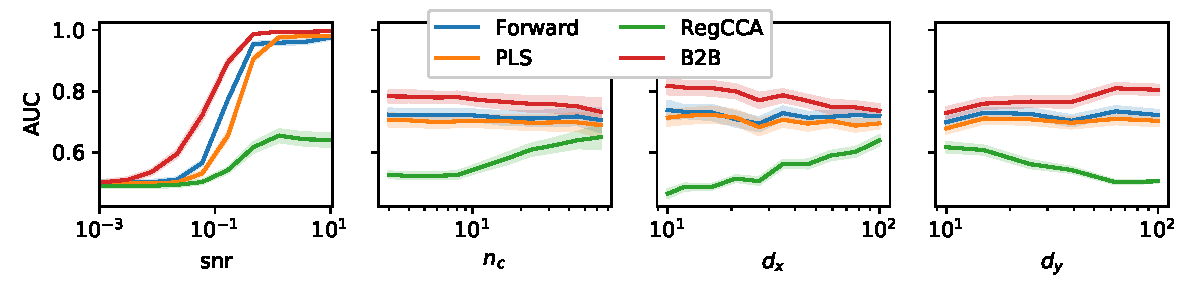
\includegraphics[width=\linewidth]{figures/auc_condition.pdf}
  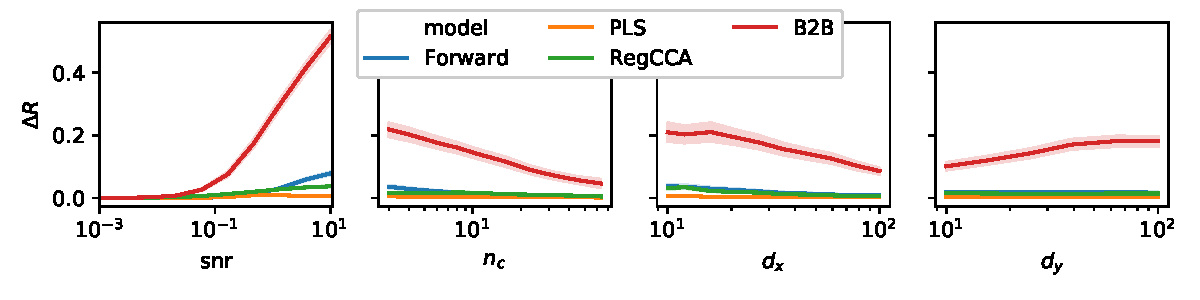
\includegraphics[width=\linewidth]{figures/r_in_condition.pdf}
  \vspace{-4ex}
  \caption{Synthetic experiments. Average AUC (top) and Feature Importance
  $\Delta R$ (bottom) when varying experimental conditions individually.
  Higher is better. B2B compares favorably in all cases.
  \label{fig:percondition}}
\end{figure}


\subsection{Evaluating Causal Discovery with held-out prediction reliability}

In most cases, $E$ is not known. The above AUC can thus not be estimated.
To address this issue, we assess the ability of each model to reliably predict
independent and identically distributed data from $Y$, given all of the $X$
features versus all-but-one feature $X_{-i}$ (i.e. 'knock-out X'). This
procedure results in two correlation metrics $R_{full}$ and $R_{knockout}$ for
each feature (for the B2B and Backward models) for each dimension of $Y$ (for
the Forward model) or each canonical dimension of $Y$ (for CCA and PLS). The
difference $\Delta R_i = R_{full}-R_{knockout}$ indicates how much each
$X_i$ improves the prediction of (a pre-defined dimension or projection of) $Y$.

We show in Appendix~\ref{appendix:feature_importance} pseudo-code to assess
feature importance for each model. For the Backward Model, feature importance
cannot be assessed as the $X$ collinearity is never
taken into account.

\subsection{Results of the synthetic experiment}

Figures~\ref{fig:percondition} (bottom) and \ref{fig:auc_plots} (right, in
Appendix) show the results of our synthetic experiment. Note that the figure
does not display each feature $i$ separately, as they are
randomly generated. $\Delta R$ represents the average of $\Delta R_i$. A
higher score means that for prediction, the model relies on individual features
rather than combinations of features. Overall both the AUC and the held-out
prediction reliability evaluations show that B2B outperforms baseline models.
